Requirements analysis is a software engineering task that has bridged the gap between system level requirements engineering and software design requirement engineering activities resulting in the specification of software’s operational characteristics (functional, data, and behavioral), that indicates software’s interface with other system elements and establishes constraints that software must meet. Gathering of requirements related to the proposed system is done. Analysis is done by comparing these requirements with working and function provided by ’existing forum system’.\\ The proposed chapter will discuss about feasibility study of the proposed system in section 2.1. The section 2.2 discuss about risk analysis. The project scheduling of system is described in section 2.3. The section 2.4 will discuss about effort allocation. Cost estimation is discussed in section 2.5. Finally the summary in last section.

\section{Feasibility Study}
% Content inside the feasibility study goes here

While considering the feasibility of any system, the system must meet its best performance by three sides i.e. technical, operational and economical feasibility. Feasibility should be considered in any organization since it helps in selection of best system for the job. It is necessary to evaluate the feasibility of the project at the early stages of software development.\\
\textbf{If project risk is great, the feasibility of product is reduced.}\\
A well designed feasibility study should provide a description of the product or service, details
of operation and working of system. A feasibility study evaluates the project potential for
success; The types of feasibility study are:
    \subsection{Technical Feasibility}
    \subsection{Operational Feasibility}
    \subsection{Economical Feasibility}

\section{Risk Analysis}
% Content if the risk analysis goes here

Risk analysis and management are actions that help a software team to understand and
manage uncertainty. A risk is a potential problem it might happen, or it may not. Risk is a uncertain event or condition that, if it occurs, has a positive or negative effect on a project’s objectives.\\
Risk always involves two characteristics: \textbf{uncertainty}- the risk may or may not happen; that is, there are no 100 percent probable risk and \textbf{loss}- if the risk becomes a reality ,unwanted consequences or losses will occur. When risks are analyzed, it is important to quantify the level of uncertainty and the degree of loss associated with each risk. The different types of risks are-\\

\begin{itemize}
    
    \item \textbf{Project Risk} threaten the project plan. That is, if project risks become real, it is likely that the project schedule will slip and that cost will increase. Project risk identify potential budgetary, schedule, personnel, resource, stakeholder, and requirements problems and their impact on a software etc.

    \item \textbf{Technical Risk} threaten the project plan. That is, if project risks become real, it is likely that the project schedule will slip and that cost will increase. Project risk identify potential budgetary, schedule, personnel, resource, stakeholder, and requirements problems and their impact on a software etc.

    
    \item \textbf{Business Risk} threaten the viability of software to be built and often jeopardize the project or the product. Candidates for the top five business risks are:
    
        \begin{enumerate}
            \item Building an excellent product or system that no one really wants\textbf{(market risk)}.
            \item Building a product that no longer fits into overall business strategy for the company\textbf{(strategic risk)}.
            \item Building a product that the sales force doesn’t understand how to sell\textbf{(sale risk)}.
            \item Losing the support of senior management due to a change in focus or a change in people\textbf{(management risk)}.
            \item  Losing budget or personnel commitment\textbf{(budget risks)}.
    
        \end{enumerate}
        
\end{itemize}
% some space is remaining herre

% Risk Analysis Table >>>>>>>>>>>
\newpage
\begin{table}[!ht]
\centering
\begin{tabular}{|l|l|l|l|}
\hline
Risk                                  & Category & Probability & Impact \\ \hline
Technology will not meet requirements & TE       & 30\%        & 1      \\ \hline
End-user resist the system            & BU       & 40\%        & 3      \\ \hline
\end{tabular}
\caption{Risk Analysis}
\end{table}

\begin{enumerate}
    \item \textbf{Catastrophic}: Failure to meet requirement would result in mission failure or increase in cost which includes schedule delay.
    \item \textbf{Critical}: Some reduction in technical performance.
    \item \textbf{Marginal}: Minimal to small reduction in technical performance.
    \item \textbf{Negligible}: No reduction in technical performance.

\end{enumerate}


\section{Project Scheduling}
\begin{figure}[h]
    \centering
    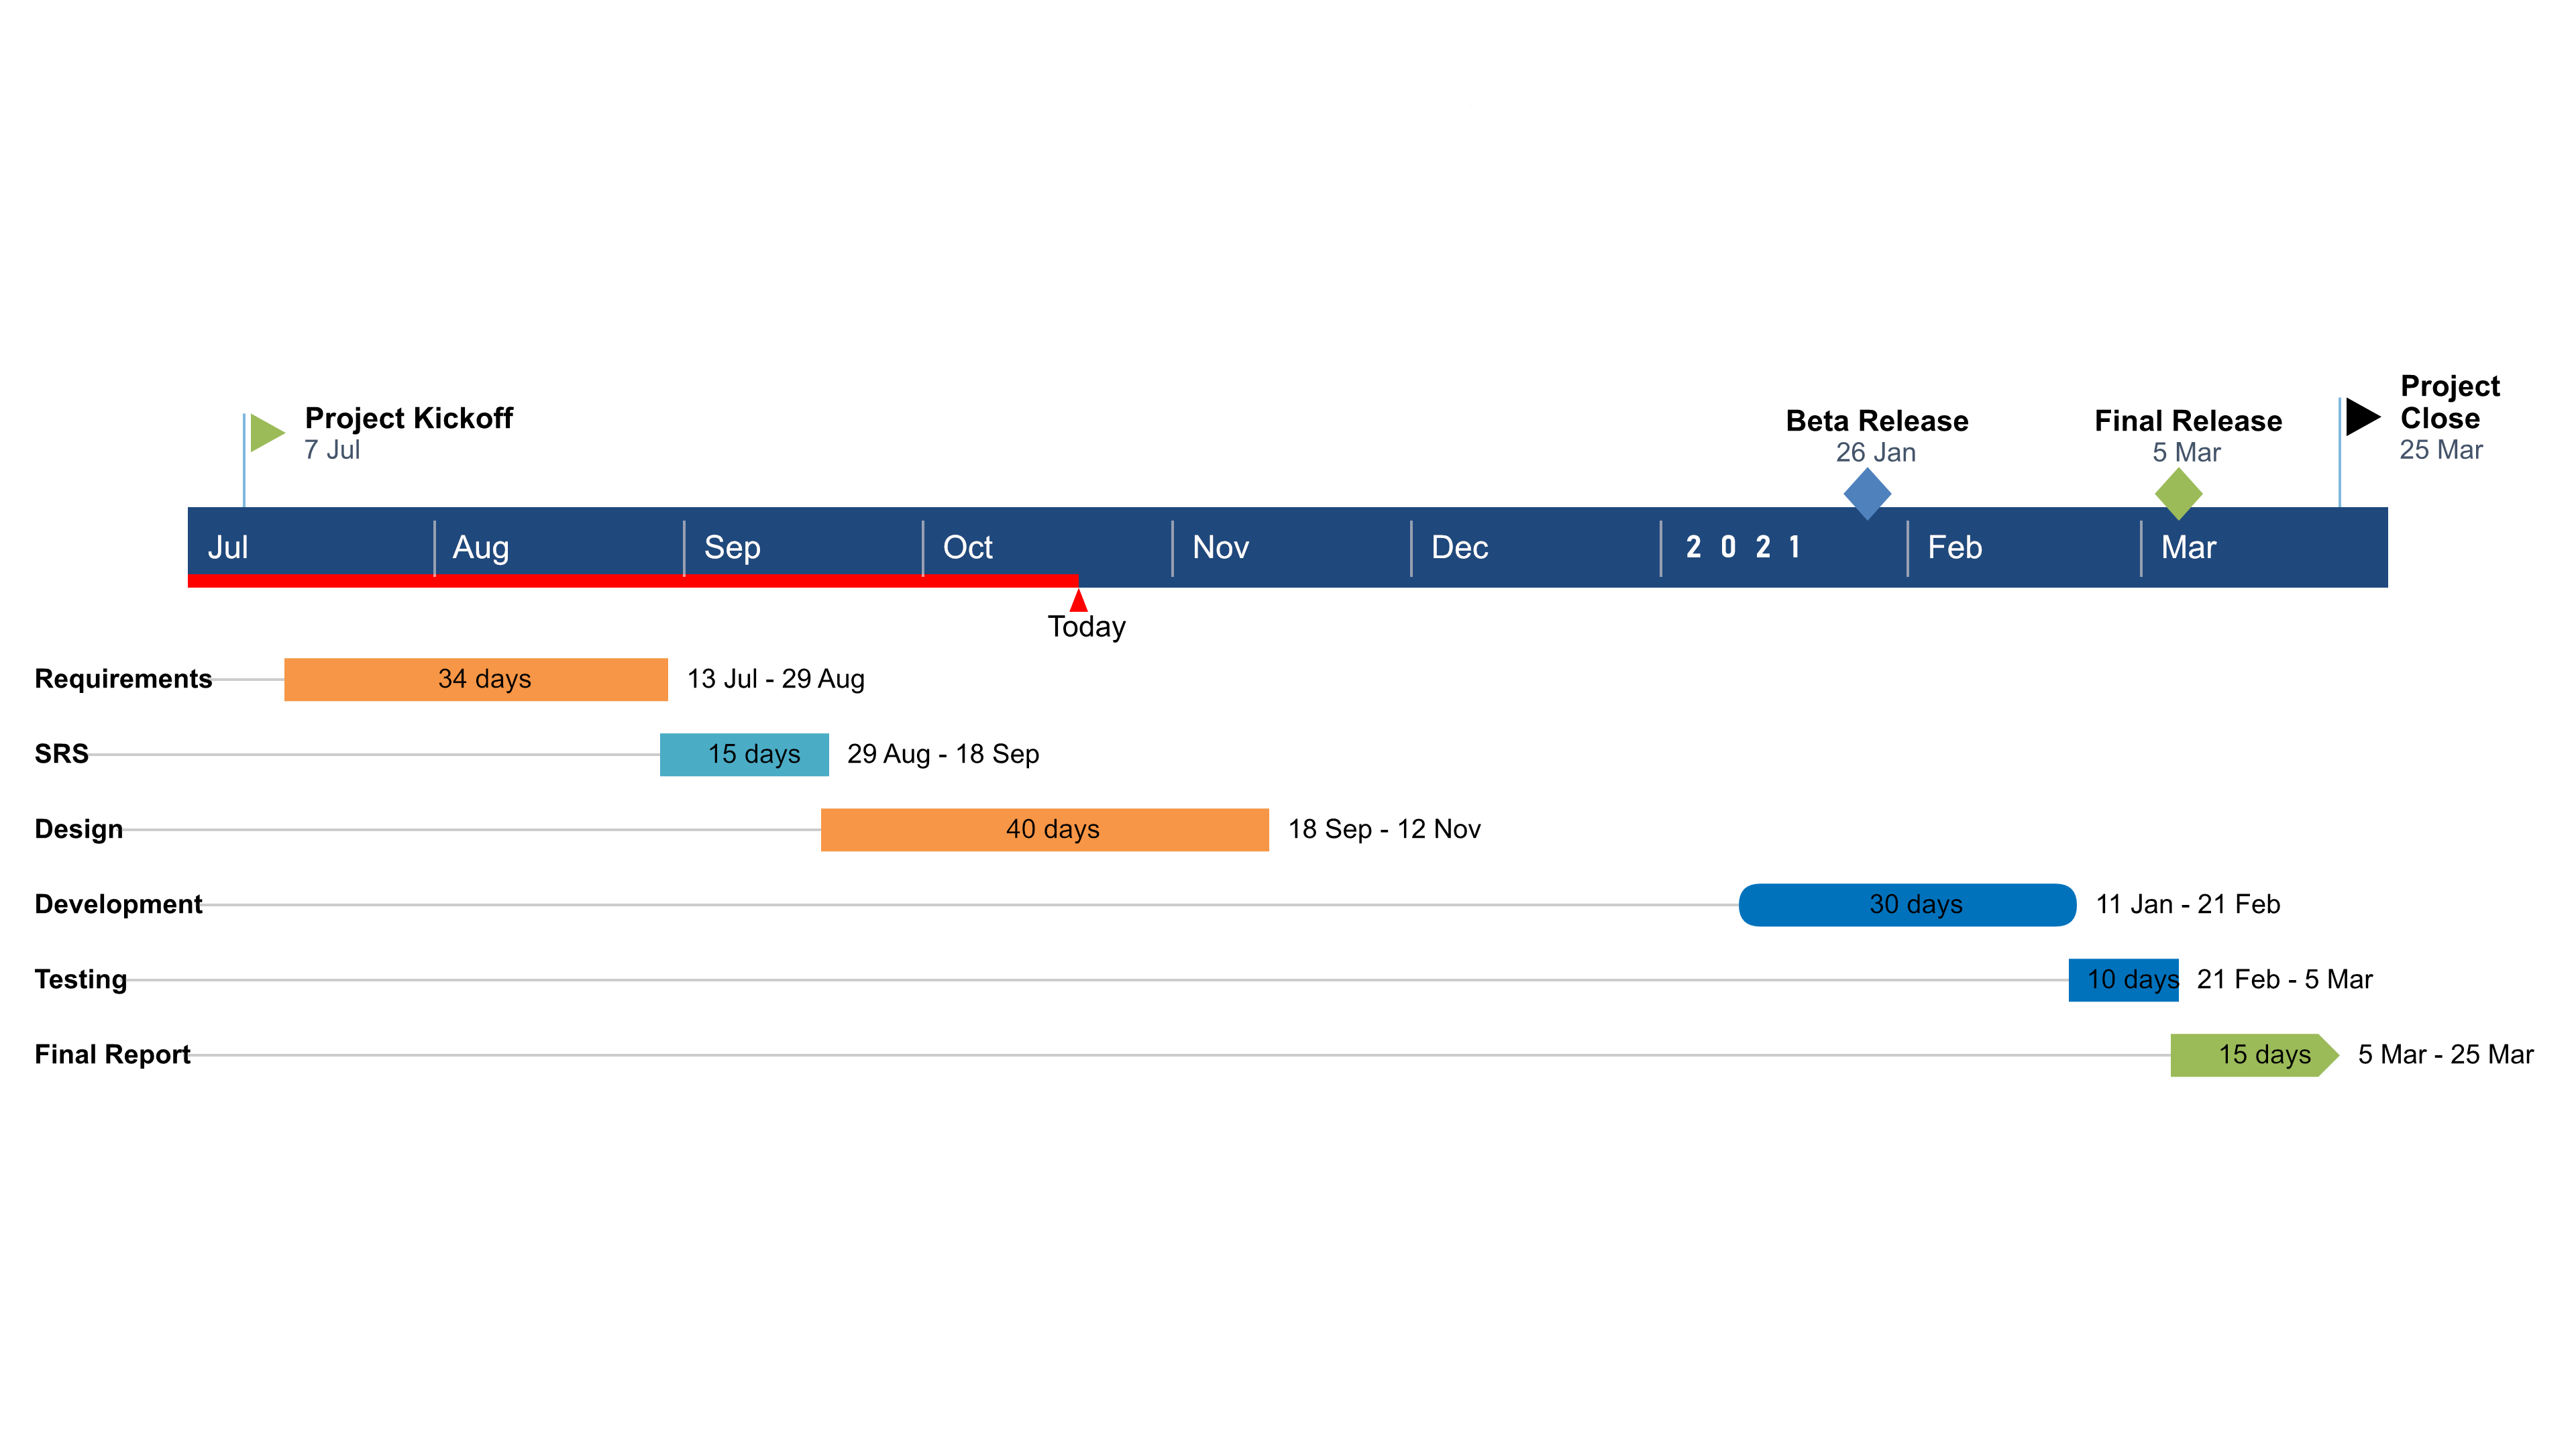
\includegraphics[width=\textwidth]{Project Planning and Management/Gantt_char_new.png}
    \caption{Gantt Chart}
    % \label{fig:my_label}
\end{figure}
\newpage

\section{Effort Allocation}
\begin{figure}[!ht]
    \centering
    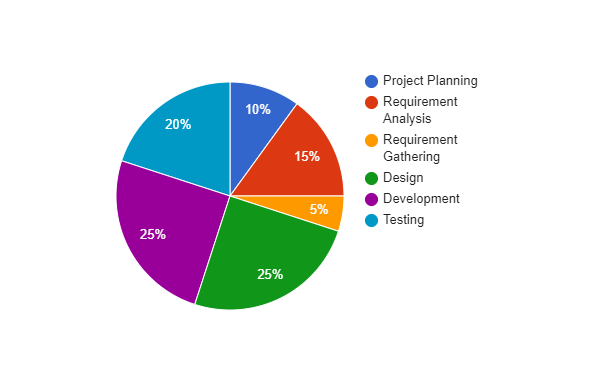
\includegraphics[width=\textwidth]{Project Planning and Management/Effort Allocation.png}
    \caption{Effort Allocation}
    \label{fig:my_label}
\end{figure}
    

\section{Cost Estimation}
    \subsection{COCOMO Model}

\section{Summary}
% Content of the summary goes here
The given chapter thoroughly describes feasibility study, risk analysis, project scheduling, effort allocation and cost estimation. The next chapter will discuss about analysis.
